\subsection{Digitale signaalbewerking}\label{sec:digitaal}

Voorbij de twee signaalverwerkingspaden van de pH-waarde en de temperatuur, komt een digitaal signaalverwerkingsblok. Dit blok, omcirkeld in \cref{fig:digitaalInSchema}  combineert de twee signalen en rekent deze om naar een pH-waarde.
\begin{figure}[!htb]
    \centering
    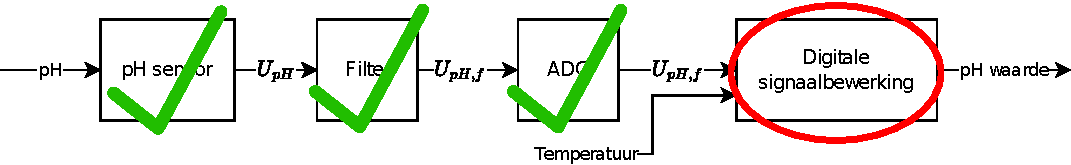
\includegraphics[width=0.95\textwidth]{signaalverwerking_digitaal}
    \caption{Het blokschema van de signaalverwerking, met de digitale signaalbewerking omcirkeld.}
    \label{fig:digitaalInSchema}
\end{figure}

Dit wordt gedaan door middel van een aantal berekeningen. Deze berekeningen zetten de door de ADC gemeten spanningen om naar een pH-waarde. Hiervoor zijn een aantal kalibratiewaardes nodig, zoals besproken in \cref{sec:werkingISFET}. Het digitale gedeelte heeft als ingang een temperatuurafhankelijke spanning $U_T$ en een pH-afhankelijke spanning $U_{pH}$. Dit is te zien in \cref{fig:digitaleBewerkingsFunctie}. Beide van deze spanningen zijn de ruwe ADC waardes die gemeten worden, en hebben dus de hoogst mogelijke resolutie, namelijk de resolutie van de ADC. Voor beide van deze waardes zal de eenheid `bit' gebruikt worden.

Om op de uiteindelijk pH-waarde te komen, wordt van de pH-afhankelijke spanning de pH-afhankelijke kalibratiespanning afgetrokken. Vervolgens wordt hier $\frac{pH_{kal}}{C_{pH}}$ bij opgeteld. Op deze manier kan er zo lang mogelijk met integers gewerkt worden die dezelfde resolutie hebben als de ingangs-ADC waarde. Het resultaat wordt vervolgens vermenigvuldigd met $C_{pH}$. Dit is de gevoeligheid van de sensor, in pH/bit.

Om de temperatuurafwijking te berekenen, wordt eerst van de temperatuurafhankelijke spanning $U_T$ de temperatuurafhankelijke kalibratiespanning $U_{T,kal}$ afgetrokken. Vervolgens wordt dit vermenigvuldigt met constante $C_T$. $C_T$ is de temperatuurafhankelijkheid van de pH-sensor, in pH/bit. Deze waarde kan afgeleid worden met de temperatuurafhankelijkheid van de pH-sensor die in de datasheet gegeven wordt in mV/K \cite{isfet}.

\begin{figure}[!htb]
    \centering
    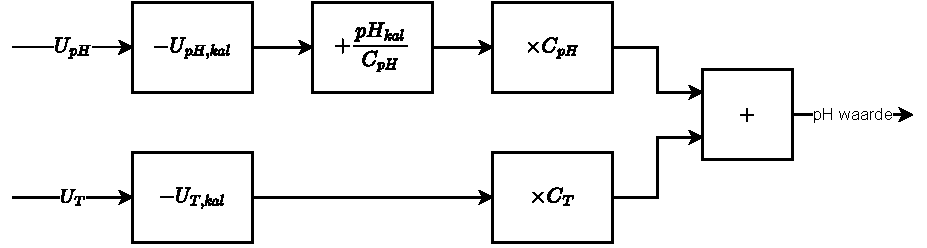
\includegraphics[width=0.95\textwidth]{digitaleBewerkingsFunctie}
    \caption{Het digitale gedeelte van de signaalbewerking.}
    \label{fig:digitaleBewerkingsFunctie}
\end{figure}
